\begin{chapter}{\label{cha:bose_gases}Introduction}
In quantum mechanics there are two classes of particle: bosons and fermions. Fermionic particles (such as electrons) follow Fermi-Dirac statistics, have half-integer spin, and obey the Pauli exclusion principle. Bosonic particles (such as photons) have integer spin, follow Bose-Einstein statistics and, unlike fermions, any number are permitted to occupy the same quantum state. In certain conditions, this latter property allows a large fraction of bosons to occupy the ground state macroscopically, a phenomenon known as Bose-Einstein condensation. Bose-Einstein condensation is as diverse as it is astonishing, appearing in all manner of physics from atomic physics to condensed matter to astrophysics, manifesting as unexpected phenomena such as superfluidity, quantised circulation and superconductivity. These effects derive directly from quantum mechanics, and so the fluids that exhibit them are known as ``quantum fluids''.

\section{Bose-Einstein condensation}\label{section:becinintro}
The roots of the original prediction of Bose-Einstein condensation lies with Satyendra Nath Bose. In 1924 Bose re-derived Planck's law of black-body radiation by developing the theory of statistical mechanics of photons. Albert Einstein went on to generalise Bose's photon distribution law to an ideal gas of $N$ massive non-interacting bosons, creating the Bose-Einstein distribution,
\begin{equation}
	f(\epsilon_i) = \frac{1}{e^{(\epsilon_i - \mu) / k_{\rm B}T} - 1},
\end{equation}
where $\epsilon_i$ is the energy of level $i$, $\mu$ is the chemical potential, $k_{\rm B}$ is the Boltzmann constant and T is the temperature. The total number of particles in the system can be written as a sum over the mean occupation of each energy level,
\begin{equation}
	N = \sum\limits_i N_i = \sum\limits_i g(\epsilon_i)f(\epsilon_i),
\end{equation}
where $N_i$ is the mean occupation of level $i$ and $g(\epsilon_i)$ is the degeneracy of level $i$. Under the Bose-Einstein distribution the occupation of the ground state diverges in the limit of zero temperature, leading to the macroscopic occupation that defines the Bose-Einstein condensate. While it is impossible to reach this limit of $T=0$ in reality, the macroscopic occupation occurs for temperatures less than a certain critical value $T<T_\lambda$. Schematically, Bose-Einstein condensation is shown in Figure \ref{fig:beclevels}.

\begin{figure}
\centering
    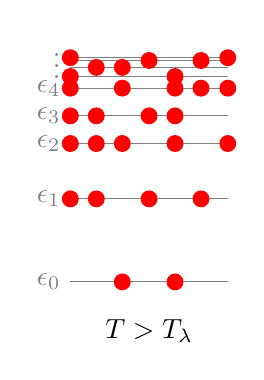
\begin{tikzpicture}
    \draw[gray] (2cm,0em) -- (0cm,0em) node[left] {$\epsilon_0$};
    \draw[gray] (2cm,3em) -- (0cm,3em) node[left] {$\epsilon_1$};
    \draw[gray] (2cm,5em) -- (0cm,5em) node[left] {$\epsilon_2$};
    \draw[gray] (2cm,6em) -- (0cm,6em) node[left] {$\epsilon_3$};
	\draw[gray] (2cm,7em) -- (0cm,7em) node[left] {$\epsilon_4$};
	\draw[gray] (2cm,7.42em) -- (0cm,7.42em) node[left] {$ $};
	\draw[gray] (2cm,7.75em) -- (0cm,7.75em) node[left] {$ $};
	\draw[gray] (2cm,8em) -- (0cm,8em) node[left] {$ $};
	\draw[gray] (2cm,8.1em) -- (0cm,8.1em) node[left] {$\vdots$};
	\draw[red,fill=red] (0.66cm,0em) circle (0.1cm);
	\draw[red,fill=red] (1.33cm,0em) circle (0.1cm);
	\draw[red,fill=red] (0cm,3em) circle (0.1cm);
	\draw[red,fill=red] (0.33cm,3em) circle (0.1cm);
	\draw[red,fill=red] (1cm,3em) circle (0.1cm);
	\draw[red,fill=red] (1.66cm,3em) circle (0.1cm);
	\draw[red,fill=red] (0cm,5em) circle (0.1cm);
	\draw[red,fill=red] (0.33cm,5em) circle (0.1cm);
	\draw[red,fill=red] (0.66cm,5em) circle (0.1cm);
	\draw[red,fill=red] (1.33cm,5em) circle (0.1cm);
	\draw[red,fill=red] (2cm,5em) circle (0.1cm);
	\draw[red,fill=red] (0cm,6em) circle (0.1cm);
	\draw[red,fill=red] (0.33cm,6em) circle (0.1cm);
	\draw[red,fill=red] (1cm,6em) circle (0.1cm);
	\draw[red,fill=red] (1.33cm,6em) circle (0.1cm);
	\draw[red,fill=red] (0cm,7em) circle (0.1cm);
	\draw[red,fill=red] (0.66cm,7em) circle (0.1cm);
	\draw[red,fill=red] (1.33cm,7em) circle (0.1cm);
	\draw[red,fill=red] (1.66cm,7em) circle (0.1cm);
	\draw[red,fill=red] (2cm,7em) circle (0.1cm);
	\draw[red,fill=red] (0cm,7.42em) circle (0.1cm);
	\draw[red,fill=red] (0.33cm,7.75em) circle (0.1cm);
	\draw[red,fill=red] (0.66cm,7.75em) circle (0.1cm);
	\draw[red,fill=red] (1cm,8em) circle (0.1cm);
	\draw[red,fill=red] (1.33cm,7.42em) circle (0.1cm);
	\draw[red,fill=red] (1.66cm,8em) circle (0.1cm);
	\draw[red,fill=red] (2cm,8.1em) circle (0.1cm);
	\draw[red,fill=red] (0cm,8.1em) circle (0.1cm);
	\draw (1cm,-1em) node[below] {$T>T_\lambda$};
    \end{tikzpicture}
    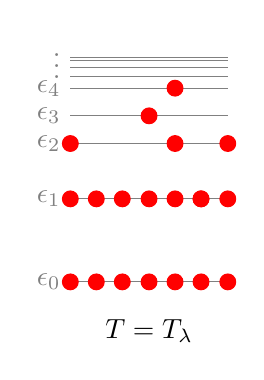
\begin{tikzpicture}
    \draw[gray] (2cm,0em) -- (0cm,0em) node[left] {$\epsilon_0$};
    \draw[gray] (2cm,3em) -- (0cm,3em) node[left] {$\epsilon_1$};
    \draw[gray] (2cm,5em) -- (0cm,5em) node[left] {$\epsilon_2$};
    \draw[gray] (2cm,6em) -- (0cm,6em) node[left] {$\epsilon_3$};
	\draw[gray] (2cm,7em) -- (0cm,7em) node[left] {$\epsilon_4$};
	\draw[gray] (2cm,7.42em) -- (0cm,7.42em) node[left] {$ $};
	\draw[gray] (2cm,7.75em) -- (0cm,7.75em) node[left] {$ $};
	\draw[gray] (2cm,8em) -- (0cm,8em) node[left] {$ $};
	\draw[gray] (2cm,8.1em) -- (0cm,8.1em) node[left] {$\vdots$};
	\draw[red,fill=red] (0cm,0em) circle (0.1cm);
	\draw[red,fill=red] (0.33cm,0em) circle (0.1cm);
	\draw[red,fill=red] (0.66cm,0em) circle (0.1cm);
	\draw[red,fill=red] (1cm,0em) circle (0.1cm);
	\draw[red,fill=red] (1.33cm,0em) circle (0.1cm);
	\draw[red,fill=red] (1.66cm,0em) circle (0.1cm);
	\draw[red,fill=red] (2cm,0em) circle (0.1cm);
	\draw[red,fill=red] (0cm,3em) circle (0.1cm);
	\draw[red,fill=red] (0.33cm,3em) circle (0.1cm);
	\draw[red,fill=red] (0.66cm,3em) circle (0.1cm);
	\draw[red,fill=red] (1cm,3em) circle (0.1cm);
	\draw[red,fill=red] (1.33cm,3em) circle (0.1cm);
	\draw[red,fill=red] (1.66cm,3em) circle (0.1cm);
	\draw[red,fill=red] (1.66cm,3em) circle (0.1cm);
	\draw[red,fill=red] (2cm,3em) circle (0.1cm);
	\draw[red,fill=red] (0cm,5em) circle (0.1cm);
	\draw[red,fill=red] (1.33cm,5em) circle (0.1cm);
	\draw[red,fill=red] (2cm,5em) circle (0.1cm);
	\draw[red,fill=red] (1cm,6em) circle (0.1cm);
	\draw[red,fill=red] (1.33cm,7em) circle (0.1cm);
	\draw (1cm,-1em) node[below] {$T=T_\lambda$};
  \end{tikzpicture}
  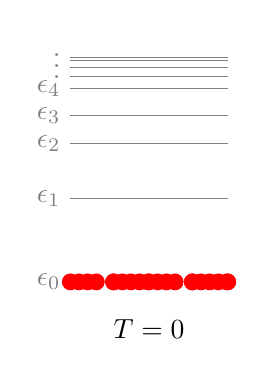
\begin{tikzpicture}
    \draw[gray] (2cm,0em) -- (0cm,0em) node[left] {$\epsilon_0$};
    \draw[gray] (2cm,3em) -- (0cm,3em) node[left] {$\epsilon_1$};
    \draw[gray] (2cm,5em) -- (0cm,5em) node[left] {$\epsilon_2$};
    \draw[gray] (2cm,6em) -- (0cm,6em) node[left] {$\epsilon_3$};
	\draw[gray] (2cm,7em) -- (0cm,7em) node[left] {$\epsilon_4$};
	\draw[gray] (2cm,7.42em) -- (0cm,7.42em) node[left] {$ $};
	\draw[gray] (2cm,7.75em) -- (0cm,7.75em) node[left] {$ $};
	\draw[gray] (2cm,8em) -- (0cm,8em) node[left] {$ $};
	\draw[gray] (2cm,8.1em) -- (0cm,8.1em) node[left] {$\vdots$};
	\draw[red,fill=red] (0cm,0em) circle (0.1cm);
	\draw[red,fill=red] (0.33cm,0em) circle (0.1cm);
	\draw[red,fill=red] (0.11cm,0em) circle (0.1cm);
	\draw[red,fill=red] (0.22cm,0em) circle (0.1cm);
	\draw[red,fill=red] (0.55cm,0em) circle (0.1cm);
	\draw[red,fill=red] (0.55cm,0em) circle (0.1cm);
	\draw[red,fill=red] (0.66cm,0em) circle (0.1cm);
	\draw[red,fill=red] (0.77cm,0em) circle (0.1cm);
	\draw[red,fill=red] (0.88cm,0em) circle (0.1cm);
	\draw[red,fill=red] (0.99cm,0em) circle (0.1cm);
	\draw[red,fill=red] (1cm,0em) circle (0.1cm);
	\draw[red,fill=red] (1.33cm,0em) circle (0.1cm);
	\draw[red,fill=red] (1.11cm,0em) circle (0.1cm);
	\draw[red,fill=red] (1.22cm,0em) circle (0.1cm);
	\draw[red,fill=red] (1.55cm,0em) circle (0.1cm);
	\draw[red,fill=red] (1.55cm,0em) circle (0.1cm);
	\draw[red,fill=red] (1.66cm,0em) circle (0.1cm);
	\draw[red,fill=red] (1.77cm,0em) circle (0.1cm);
	\draw[red,fill=red] (1.88cm,0em) circle (0.1cm);
	\draw[red,fill=red] (1.99cm,0em) circle (0.1cm);
	\draw[red,fill=red] (2cm,0em) circle (0.1cm);
	\draw (1cm,-1em) node[below] {$\phantom{T_\lambda}T=0\phantom{T_\lambda}$};
  \end{tikzpicture}
  \caption{\label{fig:beclevels}Schematic depiction of Bose-Einstein condensation. The ground state $\epsilon_0$ becomes macroscopically occupied as the temperature is reduced to below the critical temperature for condensation. In the limit of $T=0$ all bosons occupy the ground state.}
\end{figure}

Consider a gas of non-interacting bosons in thermal equilibrium at temperature $T$. The thermal de Broglie wavelength for each particle characterises the spatial extent of its localised wavepacket, and is given by
\begin{equation}
\lambda_{\rm dB} = \sqrt{\frac{2\pi \hbar^2}{mk_{\rm B}T}},
\label{eq:debroglie}
\end{equation}
where $m$ is the mass of the particle and $\hbar$ is Plank's reduced constant. The de Broglie wavelength is inversely proportional to the square root of the temperature $T$, so that at high temperatures the wavepacket of each particle is small. Here classical-like behaviour dominates the dynamics of the gas. As the temperature of the particles is reduced, the wavelength associated with the particles grows. At a critical temperature, $T_\lambda$, the wavelength for each particle becomes comparable to the average inter-particle distance and the individual characteristics of particles are no longer apparent. The particles begin to behave in a truly quantum manner, forming a degenerate gas. The critical temperature for which this process occurs marks the onset of Bose-Einstein condensation.

For a gas of identical non-interacting Bosons in a uniform three-dimensional system of volume $V$ and number density $n=N/V$, Bose-Einstein condensation occurs when $n\lambda_{\rm dB}^3 \leq \zeta(3/2)$, where $\zeta$ is the Riemann zeta function and $\zeta(3/2)\approx2.612$. By using this relation with Equation \ref{eq:debroglie} one finds the critical temperature,
\begin{equation}
T_\lambda = \frac{2\pi\hbar^2}{mk_{\rm B}} \left ( \frac{n}{\zeta(3/2)} \right )^{2/3},
\label{eq:tlambda}
\end{equation}
for the onset of Bose-Einstein condensation. The fraction of bosons condensed into the ground state can then be calculated as a function of temperature,
\begin{equation}
	\frac{N_0}{N} = 1 - \left( \frac{T}{T_\lambda}\right )^{3/2}.
\end{equation}

\section{Superfluid helium}
Many concepts relating to Bose-Einstein condensation and quantum gases were developed earlier in the context of liquid $^4$He. Liquid helium is interesting in that when cooled to very low temperatures, the liquid does not crystallise or solidify at atmospheric pressures. In fact a pressure of over $25$ atmospheres is required to solidify $^4$He, even at its lowest temperatures. 

In 1938 Kapitza, Allen and Misener observed a critical temperature (known as the lambda point) in liquid $^4$He. Below this temperature the fluid entered a new phase known as helium II. It was discovered that helium II exhibits inviscid flow (one of several remarkable properties of helium II), and the fluid was deemed a ''superfluid''.

London was the first to interpret the properties of helium II as a manifestation of Bose-Einstein condensation of helium atoms, but the idea was not widely accepted at first. The strongly-interacting liquid of helium atoms is a world away from Einstein's non-interacting gas of bosons. Instead, the two-fluid model of Landau was the first successful description of helium II hydrodynamics, wherein two fluids exist alongside one another with densities depending on the temperature: an inviscid superfluid component and a viscous normal fluid component. The superfluid component's density tents to zero as the temperature tends to the lambda point, and the normal fluid's density tends to zero as the temperature tends to zero.

\subsection{Dispersion relation and excitations}
Landau showed that superfluid behaviour can be accounted for by a dispersion relation that is linear at low momenta. Bogoliubov then showed that a weakly-interacting Bose gas supports exactly such a dispersion law. This link between bosonic gases and helium II was a strong indicator that Bose-Einstein condensation was indeed the fundamental mechanism behind superfluidity, and finally gave traction to London's theory.

\begin{figure}
	\centering
	\begin{tikzpicture}
		\begin{axis}[samples=300,ylabel near ticks,xlabel near ticks,
				width=0.4\linewidth,
				height=0.45\linewidth,
				xlabel=$p$,
				ylabel=$\epsilon$,
				xmin=0,
				xmax=13,
				ymin=0.4,
				ymax=12,
				axis line style={-Latex[round]},
				axis y line*=left,
        axis x line*=bottom,
        yticklabels={,,},
        xticklabels={,,},
				major tick length = 0.00cm]
				\addplot[mark=none,thick,domain=0:12] {x^(0.25)*((x/2-4)*sin(deg(x/2-4)) + 4)};
		\end{axis}
	\end{tikzpicture}%
	\caption{\label{fig:hedisp}The dispersion relation for superfluid $^4$He, demonstrating the spectrum of elementary excitations. The linear dispersion of phonons can be seen at at low momenta and the roton minimum at higher momenta.}
\end{figure}

The dispersion relation for liquid helium $^4$He is shown in Figure \ref{fig:hedisp}. For small momenta the relation is indeed linear. The fundamental excitations associated with this part of the relation are sound waves, known as {\it phonons}. For larger momentum, however, $\epsilon(p)$ exhibits an approximately quadratic shaped dip and local minimum. The fundamental excitations of this part of the relation are known as {\it rotons}, with the centre of the dip corresponding to the smallest possible energy of a roton, the {\it roton minimum}. 

While Bose-Einstein condensation is now known to be the driving force behind helium II superfluidity, the strong interactions inherent in liquid helium restricts the condensed fraction of helium atoms to less than $10\%$ (even in the limit of zero temperature) and so a weakly-interacting Bose gas provides only a qualitative model of helium II superfluidity.

\section{Dilute weakly-interacting atomic gases}
Gases of alkali atoms such as rubidium, sodium and lithium are ideal candidates for condensation: they are weakly-interacting, can be easily trapped magnetically, and readily cooled using lasers. When considering these gases, Einstein's ideal gas predictions provide a good estimate of the critical temperature for Bose-Einstein condensation.  However, as the gas is cooled towards the critical temperature it is necessary to avoid the transition into a liquid or solid. This can be done by reducing the atomic density such that the gas is dilute enough that elastic binary collisions in the gas dominate over three-body collisions. The required atomic densities are around $n \sim 10^{14}~{\rm cm}^{-3}$ \footnote{Compare this to the density of dry air at room temperature, $n \sim 10^{19}~{\rm cm}^{-3}$.}, and so by using Equation \ref{eq:tlambda} one predicts that the ultra-low temperatures of $T \sim 10^{-6}~{\rm K}$ are required for the onset of Bose-Einstein condensation.

The atomic binary collisions in dilute gases are characterised by the $s$-wave scattering length, $a_s$. Higher energy $p$-wave and $d$-wave scattering is suppressed. Geometrically, $a_s$ can be thought of as a measure of the effective radius of the atoms. For gases with density in the region required, $n^{1/3}a_s \ll 1$, and so $a_s$ is much smaller than the average inter-atomic distance. This implies that the gas is weakly-interacting and around $99\%$ of the atoms can become Bose-condensed, resulting in a condensate fraction much greater than the theoretical maximum for helium II. This makes ultra-cold dilute atomic gases the purest form of Bose-Einstein condensation that can also be easily controlled and manipulated in the lab.

\subsection{Experimental realisation}
The requirement of such low temperatures delayed the realisation of a true atomic Bose-Einstein condensate until 1995, when advances in atom cooling and trapping lead to the condensation of rubidium ($^{87}$Rb) by the group of Professors Carl Wieman and Eric Cornell at the University of Colorado, and sodium ($^{23}$Na) by the group of W. Ketterle at MIT. Wieman, Cornell and Ketterle were awarded the 2001 Nobel Prize in Physics for ``{\it the achievement of Bose-Einstein condensation in dilute gases of alkali atoms, and for early fundamental studies of the properties of the condensates}''.

While the advances in laser cooling, developed in the 1980s, were the main driving factor in achieving atomic Bose-Einstein condensation, in reality a combination of techniques are used in combination to reach the ultra-low temperatures required. A typical atomic condensate begins life as around $10^9$ atoms which are cooled to around 1K by a Zeeman slower: a laser beam propagating opposite to the atom flow reduces the velocity of the atoms from around $800~\rm{m/s}$ to $30~\rm{m/s}$. The atoms are transferred to a magneto-optical trap (MOT) formed by laser beams and magnetic fields and further cooled through Doppler cooling, where the Doppler effect is employed to reduce the momentum of atoms. A limit of this method is reached at around $1\,\mu$K at which point evaporative cooling is required to cool the gas even further. Here the confining trap is carefully modified so that the high energy atoms escape the system. The remaining lower energy atoms rethermalise at a reduced temperature and lower density due to the loss of atoms. Using this technique, the gas can be cooled to the nK regime. The Bose-Einstein condensate then emerges marked by a spike at the zero of the velocity distribution for the atoms, indicating a macroscopic occupation of the ground state. 

Since the first experiments in 1995, an explosion of ultra-cold atomic physics has followed. Many species of atom are now routinely condensed in the lab. The list grows continuously: many alkalis, calcium, dysprosium, strontium, ytterbium, chromium, gadolinium, metastable helium, exciton-polaritons and more. Each expanding the richness of fascinating phenomena with their unique atomic properties and range of interactions.

The experimental advances of controlling the trapping potential has allowed for direct interaction with the condensate using magnetic fields and lasers. Localised laser beams can punch a `hole' in a condensate to create almost arbitrarily shaped obstacles. Exotic trapping potentials such as ring traps, box traps, optical lattices and double-well traps can be realised with relative ease. The route has even opened to experimentation in reduced dimensionality. By significantly trapping the gas alone one dimension it is possible to make a disc shaped, effectively two dimensional condensate, useful for the study of vortex dynamics. A further trapping along a second dimension creates an elongated, effectively one dimensional condensate such that solitons are stable.

With the unique level of purity and experimental control available to researchers, weakly-interacting dilute atomic gases have become the ideal test-bed for studying Bose-Einstein condensation and for observation of quantum effects on a macroscopic scale.


\section{Macroscopic excitations: vortices and solitons}
\section{Quantum turbulence}
\end{chapter}
